\section{The planar persistent walk}\label{sec:planar}

We now return to the question of the introduction, Kagey's board in 2
dimensions. A ball moves on $\Z^2$ in the directions east, north, west and
south, numbered $0,1,2,3$ modulo $4$, with unit vectors $e_0=(1,0)$, $e_1=(0,1)$,
$e_2=-e_0$ and $e_3=-e_1$. Let $r,s\ge0$ with $\beta=2r+s>0$, and let
$0<h<1/\beta$. The first direction is uniform. After that the ball keeps its
direction with probability $p_0=1-\beta h$, turns left or right with
probability $rh$ each, and reverses with probability $sh$. This is the chain of
Example~\ref{ex:models}(iv), with $q_{j,j\pm1}=r$ and $q_{j,j+2}=s$, and its
position after $N$ steps is $Y_N=(n_0-n_2,n_1-n_3)$. So the bin is now a linear
function of the composition. In this section $N$ is even, since otherwise the
origin cannot be reached, and we allow every $h<1/\beta$. Only the path that
always goes east reaches the corner $Ne_0$, so
\[
 c_N=\Prob(Y_N=Ne_0)=\tfrac14p_0^{N-1}.
\]
We compare it with $o_N=\Prob(Y_N=0)$. Figure~\ref{fig:planarpaths} shows the
3 kinds of paths that matter.

\begin{figure}[t]
\centering
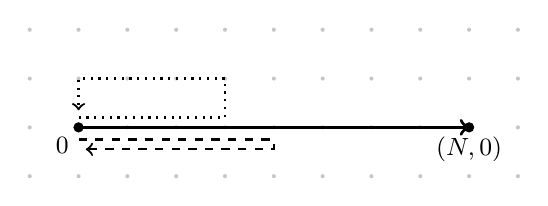
\begin{tikzpicture}[scale=0.62,font=\small]
 \foreach \x in {-1,...,9} \foreach \y in {-1,...,2} \fill[gray!45] (\x,\y) circle (1.2pt);
 \draw[very thick,->] (0,0) -- (8,0);
 \draw[thick,dashed,->] (0,-0.25) -- (4,-0.25) -- (4,-0.45) -- (0.15,-0.45);
 \draw[thick,dotted,->] (0,0.2) -- (3,0.2) -- (3,1) -- (0,1) -- (0,0.35);
 \fill (0,0) circle (3pt) node[below left] {$0$};
 \fill (8,0) circle (3pt) node[below] {$(N,0)$};
\end{tikzpicture}
\caption{Paths of $N=8$ steps. The only path to the corner $(N,0)$ never
switches (solid). A path to the origin either stays on one axis and only
reverses (dashed), or it turns and then uses all 4 directions (dotted).}
\label{fig:planarpaths}
\end{figure}

We write $u=sh/p_0$, $v=rh/p_0$ and $w=\beta h/p_0=2v+u$, so $1+w=1/p_0$. These
are the odds of a reversal, of a turn to a given side and of any switch, as in
the shared notation $u=q/p$. We use $S_N$, $u_N$, $p_N$, $z_N=N(1-p_N)$ and
$c_0$ from Section~\ref{sec:notation}. As $N$ is even, $S_N(u)$ is the sum of
$u^j$ over the words with $N/2$ letters of each of 2 kinds, where $j$ is the
number of switches. It has nonnegative coefficients and no constant term, so it
increases strictly on $[0,\infty)$.

\emph{The answer at first order.} Face selection predicts the answer, up to
powers of $\log N$. Let $h=\tau\log N/N$. The corner is the vertex $\{0\}$,
which has exit rate $\beta$, so $c_N$ is about $N^{-\beta\tau}$. A vertex, a
face with 3 directions, or a face with 2 adjacent ones misses the opposite of
one of its directions, so it cannot reach the origin. On the axis $\{0,2\}$,
which has exit rate $2r$, the origin is the single composition
$(N/2,0,N/2,0)$, of probability about $N^{-(2r\tau+1)}$. On the full face a
single composition has probability about $N^{-3}$, but about $N/2$
compositions $(a,b,a,b)$ end at the origin, and together they give about
$N^{-2}$. So the origin should beat the corner when $\beta\tau>\min(2r\tau+1,2)$,
that is, when $\tau>\tau^*=\min(2/\beta,1/s)$. At $\tau^*$ the axes win if
$s>2r$ and the full face wins if $s<2r$. This is only a heuristic, since it
applies Theorem~\ref{thm:first} to a linear function of the composition, which
we have not proved in general. Theorem~\ref{thm:planar-first} proves the
conclusion directly, and Theorem~\ref{thm:planar-rev} finds the crossing up to
$O(N^{-\gamma})$ when reversals dominate. The tool is a decomposition of a path
into 3 independent levels.

\begin{lemma}[3 levels]\label{lem:threelevel}
Write a sequence of directions as its number $m$ of switches, its skeleton $Z=(Z_0,\dots,Z_m)$,
which lists the directions of the runs so that $Z_t\ne Z_{t-1}$, and its run lengths
$\ell=(\ell_0,\dots,\ell_m)$, which form a composition of $N$ into $m+1$ positive parts. This is a
bijection, and $Y_N=\sum_{t=0}^m\ell_te_{Z_t}$. Under the walk, \textup{(a)} $m$ has the law
$\mathrm{Bin}(N-1,\beta h)$. Given $m$, \textup{(b)} $Z$ and $\ell$ are independent, \textup{(c)}
$Z$ is the random walk on $\Z_4$ with uniform $Z_0$ whose independent increments are $\pm1$ with
probability $r/\beta$ each and $2$ with probability $s/\beta$, and \textup{(d)} $\ell$ is uniform on
the $\binom{N-1}m$ compositions.
\end{lemma}

\begin{proof}
Put $q(\pm1)=r$ and $q(2)=s$. The sequence with data $(m,Z,\ell)$ has probability
\[
 \frac14p_0^{N-1-m}\prod_{t=1}^mh\,q(Z_t-Z_{t-1})
 =\binom{N-1}m(\beta h)^mp_0^{N-1-m}\cdot\frac14\prod_{t=1}^m\frac{q(Z_t-Z_{t-1})}\beta
 \cdot\binom{N-1}m^{-1}.
\]
For fixed $m$ the middle factor is the probability of $Z$ under the walk in (c), so it sums to $1$
over the skeletons, and the last factor sums to $1$ over the compositions. So the 3 factors are the
laws in (a), (c) and (d), and the product form gives (b).
\end{proof}

\begin{proposition}[exact decomposition and a unique crossing]\label{prop:decomp}
Let $N\ge2$ be even and $0<h<1/\beta$. Let $o^{(0)}_N$ and $o^{(4)}_N$ be the probabilities that
$Y_N=0$ and the walk never turns, and that $Y_N=0$ and the walk uses all 4 directions. Then
$o_N=o^{(0)}_N+o^{(4)}_N$,
\[
 o^{(0)}_N=2S_N(u)\,c_N,\qquad 0\le o^{(4)}_N\le\frac{w^2}{2p_0}\bigl(1-p_0^N\bigr).
\]
Equivalently, $o_N/c_N=2S_N(u)+E_N$ with $0\le E_N\le2w^2\bigl((1+w)^N-1\bigr)$. Also, $o_N/c_N$
is a polynomial in $v$ and $u$ with nonnegative coefficients and no constant term. If $s>0$, or if
$s=0$ and $N\ge4$, it increases strictly in $h$ from $0$ at $h=0$ to $\infty$ as $h\uparrow1/\beta$.
So there is exactly one $h^*_N\in(0,1/\beta)$ with $o_N=c_N$, and the corner is more likely than the
origin exactly when $h<h^*_N$.
\end{proposition}

In words: the origin mass splits exactly into the axis part, which is twice the
middle bin of Kagey's board measured against its endpoint, and a part from
paths with all 4 directions, which is small when $w$ is small. The ratio
$o_N/c_N$ grows with the switching rate, so the corner and the origin cross
exactly once, at every even $N\ge4$.

\begin{proof}
An origin path with no turn stays on the axis of its first step. An origin path that turns uses both
axes, and since $n_0=n_2$ and $n_1=n_3$ at the origin, it uses all 4 directions. So every origin
path is of exactly one of the 2 kinds. The origin paths on the axis $\{0,2\}$ are the paths with
$n_0=n_2=N/2$, and the path that always goes east has probability $c_N$. So
Proposition~\ref{prop:pair} with $a=s$ and $q=\beta$, for the pairs $\{0,2\}$ and $\{1,3\}$, gives
$o^{(0)}_N=2S_N(u)c_N$. The bound on $o^{(4)}_N$ follows from Lemma~\ref{lem:threelevel} and a count
of the run lengths that bring a skeleton back to the origin. We prove it in
Appendix~\ref{app:planar}. Dividing by $c_N$ gives the form with $E_N$.

A path with $a$ turns and $b$ reversals has probability $\frac14p_0^{N-1-a-b}(rh)^a(sh)^b=c_Nv^au^b$.
So $o_N/c_N$ is the sum of $v^au^b$ over the origin paths, and $a+b\ge1$ for each of them. Both $u$
and $v$ are nondecreasing in $h$, and each of them with a positive rate increases strictly to
$\infty$ as $h\uparrow1/\beta$. If $s>0$, the path that goes east $N/2$ times and then west gives
the term $u$. If $s=0$ and $N\ge4$, then $r>0$, and a path whose 4 runs go east, north, west and
south, with lengths $a,b,a,b\ge1$, gives the term $v^3$. This proves the claims on monotonicity and
the limits. For $s=0$ and $N=2$ the origin cannot be reached.
\end{proof}

The identity and the unique crossing for $s>0$ are checked in Lean (Section~\ref{sec:verify}). We
write $T^*_N=Nh^*_N$ and $u^*_N=sh^*_N/(1-\beta h^*_N)$. At the crossing $o_N=c_N$, so
$2S_N(u^*_N)=o^{(0)}_N/o_N$ there. We call it the zero-turn share of the origin mass.

We compare $S_N$ with Bessel functions by the uniform Bessel bound of~\cite{paperA}. Put
$\psi(z)=z(I_0(z)+I_1(z))$. In our notation that bound says that for every $N\ge2$ and $z>0$
\begin{equation}\label{eq:planar-bessel}
 \Bigl(1-\frac{z(z+2)}{2N}\Bigr)\psi(z)\le\frac N2\,S_N\Bigl(\frac zN\Bigr)\le\psi(z).
\end{equation}
Since $I_0'=I_1$ and $(zI_1)'=zI_0$, we have $\psi'=\psi+I_0$, so $(\log\psi)'\ge1$.

\begin{theorem}[first order]\label{thm:planar-first}
Fix $r>0$ and $s\ge0$, put $\tau^*=\min(2/\beta,1/s)$ with $1/0=\infty$, and let $N\to\infty$
through even integers.
\begin{enumerate}[(a)]
\item Fix $\tau>0$ and put $h=\tau\log N/N$. If $\tau<\tau^*$, then $o_N/c_N\le N^{-\gamma}$ for
some $\gamma>0$ and all large $N$. If $\tau>\tau^*$, then $o_N/c_N\ge N^{\gamma}$ for some
$\gamma>0$ and all large $N$.
\item $T^*_N/\log N\to\tau^*$.
\item If $s>2r$, then $2S_N(u^*_N)\to1$, so the origin mass at the crossing comes from the 2 axes,
half from each. If $s<2r$, then $2S_N(u^*_N)\le N^{-\gamma}$ for some $\gamma>0$ and all large $N$,
so it comes from the paths that use all 4 directions.
\end{enumerate}
\end{theorem}

In words, the heuristic above is right: the crossing sits at $T\approx\tau^*\log
N$, and at the crossing the origin is reached through the axes when reversals
dominate and through all 4 directions when turns dominate.

\emph{Idea of the proof.} The proof is in Appendix~\ref{app:planar}. The upper
bound in (a) follows from Proposition~\ref{prop:decomp} and
\eqref{eq:planar-bessel}. For the lower bound when $\beta\tau>2$ we count
balanced skeletons with Lemma~\ref{lem:threelevel}, and they give $o^{(4)}_N$ of
order at least $N^{-2}T^{-1/2}$. Part (b) follows from (a) and the monotonicity
in Proposition~\ref{prop:decomp}. For $r=0$ the same limit $1/s$ follows from
Theorem~\ref{thm:planar-rev}(c).

When reversals dominate, the crossing is the crossing of~\cite{paperA} for $N/2$ steps. We write
$z_{N/2}=\frac N2(1-p_{N/2})$ for it, and put
\[
 \mathcal A(\Lambda)=\Lambda-\tfrac12\log\Lambda+c_0
 +\frac{\frac14\log\Lambda-\frac12c_0+\frac18}{\Lambda},
\]
so that the third-order expansion of $z_N$ in~\cite{paperA} reads
$z_N=\mathcal A(L)+O((\log L)^2/L^2)$.

\begin{theorem}[reversals dominate]\label{thm:planar-rev}
\begin{enumerate}[(a)]
\item Let $s>0$. For all even $N\ge2$ and $0<h<1/\beta$,
\[
 \frac{o_N}{c_N}=2S_N(u)\bigl(1+\varepsilon_N(h)\bigr),\qquad
 0\le\varepsilon_N(h)\le\frac{w^2(1+w)^N}{S_N(u)}.
\]
\item Let $r\ge0$ and $s>2r$, let $N\to\infty$ through even integers, and let
$0<\gamma<\min(1,(s-2r)/s)$. Then
\[
 \varepsilon_N(h^*_N)=O\bigl((\log N)^{3/2-r/s}N^{-(s-2r)/s}\bigr),\qquad
 Nu^*_N=z_{N/2}+O(N^{-\gamma}).
\]
\item Under the hypotheses of (b), $sT^*_N=z_{N/2}+O(N^{-\gamma})$. Hence
\[
 sT^*_N=\mathcal A(L-\log2)+O\Bigl(\frac{(\log L)^2}{L^2}\Bigr),\qquad
 sT^*_N-z_N=-\log2+\frac{\log2}{2L}+O\Bigl(\frac{(\log L)^2}{L^2}\Bigr).
\]
\end{enumerate}
\end{theorem}

In words: when reversals dominate, the planar walk at its crossing behaves like
Kagey's board with half as many steps, and its crossing is smaller than
Kagey's by $\log2$ in the limit. Here is why. At the crossing $o_N\approx
o^{(0)}_N=2S_N(u)c_N$, so the 2 axes double the mass at the origin. By
\eqref{eq:planar-bessel}, applied with $N$ and with $N/2$ steps, the equations
$2S_N(z/N)=1$ and $S_{N/2}(z/(N/2))=1$ both say that $\psi(z)\approx N/4$. So
doubling $S_N$ has the same effect as halving $N$.

\begin{proof}
(a) Since $s>0$, $S_N(u)\ge2u>0$. Divide Proposition~\ref{prop:decomp} by $2S_N(u)$. Then
$\varepsilon_N(h)=E_N/(2S_N(u))$ and $E_N\le2w^2(1+w)^N$.

(b) Write $u^*=u^*_N$, $z^*=Nu^*$ and $E^*=E_N(h^*_N)$. At the crossing
Proposition~\ref{prop:decomp} gives $2S_N(u^*)+E^*=1$. So $S_N(u^*)\le\frac12<S_N(u_N)$, and
$u^*<u_N$. Put $w_N=\beta u_N/s$. Since $w\mapsto2w^2(1+w)^N$ is increasing,
$E^*\le\eta_N:=2w_N^2(1+w_N)^N$. By the second-order expansion of $z_N$ in~\cite{paperA},
$Nu_N=z_N/p_N=L-\frac12\log L+O(1)$. So $(1+w_N)^N\le e^{Nw_N}=O(N^{\beta/s}L^{-\beta/(2s)})$ and
$w_N^2=O(L^2/N^2)$. As $\beta/s-2=-(s-2r)/s$ and $2-\beta/(2s)=\frac32-\frac rs$, this gives
$\eta_N=O(L^{3/2-r/s}N^{-(s-2r)/s})$, which tends to $0$. Then
$\varepsilon_N(h^*_N)=E^*/(1-E^*)\le\eta_N/(1-\eta_N)$.

Next let $z'=\frac N2u_{N/2}$, so that $S_{N/2}(2z'/N)=1$. By \eqref{eq:planar-bessel} with
$N/2$ steps, $\frac N4\le\psi(z')\le\frac N4(1-\delta'_N)^{-1}$ with $\delta'_N=z'(z'+2)/N$. By
\eqref{eq:planar-bessel} with $N$ steps and $\frac12(1-\eta_N)\le S_N(u^*)\le\frac12$, we get
$\frac N4(1-\eta_N)\le\psi(z^*)\le\frac N4(1-\delta_N)^{-1}$ with $\delta_N=z^*(z^*+2)/(2N)$. Both $z'$
and $z^*<Nu_N$ are $O(L)$, so $\delta_N,\delta'_N=O(L^2/N)$. As $(\log\psi)'\ge1$,
$\lvert z^*-z'\rvert\le\lvert\log\psi(z^*)-\log\psi(z')\rvert=O(\eta_N+L^2/N)$. Finally
$z_{N/2}=z'/(1+u_{N/2})=z'+O(L^2/N)$. So $z^*-z_{N/2}=O(\eta_N+L^2/N)$, which is $O(N^{-\gamma})$.

(c) Since $h^*_N=u^*/(s+\beta u^*)$, we have $sT^*_N=z^*/(1+\beta u^*/s)=z^*+O(L^2/N)$, as
$u^*<u_N=O(L/N)$. With (b) this gives $sT^*_N=z_{N/2}+O(N^{-\gamma})$. The third-order expansion of
$z_N$ in~\cite{paperA}, for $N/2$ steps and for $N$ steps, gives
$z_{N/2}=\mathcal A(L-\log2)+O((\log L)^2/L^2)$ and $z_N=\mathcal A(L)+O((\log L)^2/L^2)$. The last
term of $\mathcal A$ has derivative $O(\log L/L^2)$ near $L$, so
\[
 \mathcal A(L-\log2)-\mathcal A(L)=-\log2-\tfrac12\log\Bigl(1-\frac{\log2}L\Bigr)
 +O\Bigl(\frac{\log L}{L^2}\Bigr)=-\log2+\frac{\log2}{2L}+O\Bigl(\frac{\log L}{L^2}\Bigr).
\qedhere
\]
\end{proof}

For $(r,s)=(0.1,1)$ the difference $sT^*_N-z_N$ is $-0.6317$ at $N=640$ and $-0.6493$ at
$N=10240$, while the first 2 terms in (c) give $-0.6395$ and $-0.6556$ (Figure~\ref{fig:planar}(a)).
When turns dominate, the origin mass is carried by the paths with all 4 directions, and we need
their local limit.

\begin{remark}[when turns matter, proof omitted]\label{rem:planar-turns}
Let $r>0$ and $s\ge0$, let $N\to\infty$ through even integers, and let $T=Nh\to\infty$ with
$T\le N^{1/8}$. Then $N^2o^{(4)}_N=\frac{2(r+s)}\pi T(1+o(1))$. This is twice the density at $0$ of
a centered Gaussian vector with covariance $\frac{N^2}{2(r+s)T}I_2$, and the factor $2$ appears
because $Y_N$ lies on a sublattice of index $2$. If $s<2r$, it gives
\[
 \beta T^*_N+\log T^*_N=2L+\log\frac\pi{8(r+s)}+o(1),\qquad\text{or}\qquad
 \beta T^*_N=2z_N+\log\frac\beta{2(r+s)}+o(1).
\]
For $r=s=1$ the bold curve of Figure~\ref{fig:program} solves the first equation without its
$o(1)$ term. The coefficient of $\log T^*_N$ is $1$ and not $\frac12$, because the origin is a point of a
2-dimensional local limit. Still $T^*_N=\tau^*[L-\frac12\log L+O(1)]$ for every $s\ge0$. At the
switch $s=2r$ the zero-turn share tends to $2\sqrt2/(\sqrt2+\sqrt5)=0.7749$, and the term
$\log((\sqrt5-\sqrt2)/(\sqrt5+\sqrt2))$ is added to the right side of the first equation. The
approach is slow. At $N=10240$ the zero-turn share is $0.7650$ for $(r,s)=(0.5,1)$ and still
$0.1051$ for $(1,1)$ (Figure~\ref{fig:planar}(b)). With turns only ($s=0$), we rotate the lattice
by $45^\circ$. If $Y_N=(Y^{(1)},Y^{(2)})$, then $Y^{(1)}+Y^{(2)}$ and $Y^{(1)}-Y^{(2)}$ move by
$\pm1$ at each step, and their sign words are 2 copies of the walk of~\cite{paperA} that never
switch at the same step. So $Y_N=0$ exactly when both words are balanced, which is the lattice form
of the factorization in~\cite[Eq.~(36)]{angelani2022}. A union bound over the pairs of balanced
words that switch at a common step then gives $rT^*_N=z_N+O((\log N)^4/N)$. The other proofs use
Lemma~\ref{lem:threelevel}, a local limit for the run lengths given the skeleton and a martingale
central limit theorem~\cite{hallheyde1980} for the skeleton. We omit the details.
\end{remark}

\begin{figure}[t]
\centering
\includegraphics[width=\textwidth]{fig_planar}
\caption{(a) The exact crossing of the planar walk with $(r,s)=(0.1,1)$, written as
$sT^*_N-z_N$ with $z_N=N(1-p_N)$, for $N=40,80,\dots,10240$. The dashed curve is
$-\log2+\log2/(2L)$ from Theorem~\ref{thm:planar-rev}(c), and the dotted line is its limit $-\log2$.
(b) The zero-turn share $2S_N(u^*_N)$ of the origin mass at the crossing. It tends to $1$ for
$s>2r$ and to $0$ for $s<2r$ (Theorem~\ref{thm:planar-first}), and by
Remark~\ref{rem:planar-turns} (proof omitted) to $2\sqrt2/(\sqrt2+\sqrt5)=0.7749$ at the switch
$s=2r$. For $(r,s)=(1,0)$ there are no reversals and
the share is $0$ for every $N$. The pair $(0.3,1)$ was computed up to $N=640$.}
\label{fig:planar}
\end{figure}
